\chapter{Conceitos Básicos}
\label{chapter:basicConcepts}



%----------NOTATION
\section{Algumas palavras sobre a notação}

Um dos principais objectivos deste texto é reunir, corrigir e harmonizar a
informação necessária para compreender os mecanismos internos de Monero. Ao
mesmo tempo, queremos apresentar a matéria de forma construtiva: cada símbolo
deve conservar o seu papel enquanto acrescentamos uma peça de cada vez.

Salvo indicação em contrário, adoptamos as seguintes convenções:

\begin{itemize}
\item letras minúsculas para inteiros, escalares, sequências de bits e valores
simples;
\item letras maiúsculas para pontos de curva elíptica e objectos compostos.
\end{itemize}

Tentamos também reservar os mesmos símbolos para os mesmos objectos. Um
gerador de curva será normalmente \(G\), a ordem do seu subgrupo será \(l\), e
um par de chaves privada e pública será escrito \(k/K\), respectivamente.

A apresentação é deliberadamente {\em conceptual}. Um leitor de ciência da
computação poderá sentir falta da representação exacta de certos objectos ou
dos pormenores de uma implementação; um estudante de matemática poderá desejar
mais álgebra abstracta. Daremos esses pormenores quando forem necessários ao
raciocínio, sem os deixar esconder a construção principal.

%Beyond that, we have aimed at being {\em conceptual} in our presentation of algorithms and schemes. A reader with a computer science background may feel we have neglected questions like the bit representation of items, or, in some cases, how to carry out concrete operations. Moreover, students of mathematics may find we disregarded explanations of abstract algebra.

Um objecto simples, como um inteiro ou uma sequência de caracteres, pode ser
codificado como uma sequência de bits. A ordem dos bytes, ou {\em endianness},
é essencial para uma implementação interoperável, mas raramente altera as
ideias estudadas neste capítulo; quando importar, será indicada.
%However, we don’t see this as a loss. A simple object such as an integer or a string can always be represented by a bit string. So-called `endianness' is rarely relevant, and is mostly a matter of convention for our algorithms.
%\footnote{In computer memory, each byte is stored in its own address (an address is akin to a numbered slot, which a byte can be stored in). A given `word' or variable is referenced by the lowest address of its bytes. If variable $x$ has 4 bytes, stored in addresses 10-13, address 10 is used to find $x$. The way bytes of $x$ are organized in its set of addresses depends on {\em endianness}, although each individual byte is always and everywhere stored the same way within its address. Basically, which end of $x$ is stored in the reference address? It could be the {\em big end} or {\em little end}. Given $x = $ 0x12345678 (hexadecimal, 2 hexadecimal digits occupy 1 byte e.g. 8 binary digits a.k.a. bits), and an array of addresses \{10, 11, 12, 13\}, the big endian encoding of $x$ is \{12, 34, 56, 78\} and the little endian encoding is \{78, 56, 34, 12\}. \cite{endianness}}

Um ponto de curva elíptica escreve-se habitualmente como um par \((x,y)\), mas
isso não obriga a transmiti-lo como dois inteiros completos. Na secção
\ref{point_compression_section} veremos como uma coordenada e um bit bastam
para codificar os pontos que nos interessam. Sempre que contarmos bytes,
assumiremos essa compressão.

As funções hash\marginnote{src/crypto/ {\tt keccak.c}} serão por vezes usadas
sem declarar um algoritmo específico. Monero emprega uma variante de
\(\mathit{Keccak}\), cuja construção interna não é necessária para a teoria
deste capítulo\footnote{\label{kekkak_note}O algoritmo Keccak serve de base ao
standard NIST {\em SHA-3} \cite{nist-sha3}.}.
%The Keccak hashing algorithm forms the basis for the NIST standard {\em SHA-3} \cite{nist-sha3}.}

Chamaremos simplesmente {\em função hash} a uma função de dispersão
criptográfica. Ela recebe uma mensagem \(\mathfrak{m}\) de comprimento variável
e devolve uma sequência \(h\) de comprimento fixo. É determinística: a mesma
entrada dá sempre a mesma saída. Pretende-se, contudo, que as saídas se pareçam
com escolhas uniformes e imprevisíveis, que seja computacionalmente difícil
recuperar uma entrada a partir da sua hash e que seja difícil encontrar duas
entradas distintas com a mesma saída. O chamado {\em efeito avalanche} faz com
que uma pequena alteração da entrada possa mudar muitos bits da saída.

Aplicaremos funções hash a inteiros, sequências de caracteres, pontos de curva
e combinações desses objectos. Isso significa que primeiro se usa uma
codificação binária inequívoca e, quando há vários objectos, uma concatenação
inequívoca. Uma hash é originalmente uma sequência de bits; para a usar como
escalar ou ponto de curva é ainda necessária uma conversão apropriada, que
indicaremos quando for relevante.

%----------MODULAR ARITHMETIC
\section{Aritmética modular}
\label{sec:modular-arithmetic}

A maior parte da criptografia moderna começa com aritmética modular. Fixemos
um módulo \(n>1\). Para qualquer inteiro \(a\), a operação
\[
c=a\bmod n
\]
devolve o único resto \(c\) que satisfaz
\[
a=qn+c,\qquad 0\leq c<n,
\]
para algum inteiro \(q\). O símbolo \(\bmod\) designa aqui uma operação. Quando
queremos afirmar que dois inteiros deixam o mesmo resto, escrevemos antes a
congruência \(a\equiv c\pmod n\).

Os restos nunca são negativos. Em particular, se \(0<a<n\), então
\((-a)\bmod n=n-a\). Nos casos de fronteira convém não abreviar: se
\(a\bmod n=0\), também \((-a)\bmod n=0\). A fórmula que cobre todos os casos é
\[
(-a)\bmod n=\bigl(n-(a\bmod n)\bigr)\bmod n.
\]


\subsection{Adição e multiplicação modular}
\label{subsec:modular-addition-multiplication}

Ao implementar estas operações, reduzir resultados intermédios evita inteiros
desnecessariamente grandes. Suponhamos, por exemplo, que queremos calcular
\((29+87)\bmod 99\), mas que não desejamos formar primeiro \(116\). Para
restos \(0\leq a,b<n\), pomos \(x=n-a\):
\begin{itemize}
    \item se \(b<x\), então \((a+b)\bmod n=a+b\);
    \item se \(b\geq x\), então \((a+b)\bmod n=b-x\).
\end{itemize}
No exemplo, \(x=70\) e obtemos directamente \(87-70=17\). A igualdade no
segundo caso é importante: quando \(a+b=n\), o resto é zero.

Podemos repetir esta adição segura para calcular uma multiplicação modular. O
algoritmo chama-se {\em duplica-e-adiciona}. Por exemplo,
\[
(7\cdot 8)\bmod 9=(8+8+8+8+8+8+8)\bmod 9=2.
\]
Agrupando parcelas iguais,
\[
(8+8)+(8+8)+(8+8)+8
\]
e depois
\[
[(8+8)+(8+8)]+(8+8)+8,
\]
podemos reutilizar cada duplicação em vez de repetir todo o trabalho.
\footnote{A vantagem torna-se clara para multiplicadores grandes: a adição
repetida exige um número de operações proporcional ao multiplicador, enquanto
duplica-e-adiciona exige apenas um número proporcional ao seu comprimento em
bits.}
%The effect of double-and-add becomes apparent with large numbers. For example, with $2^{15} * 2^{30}$ straight addition would require about $2^{15}$ $+$ operations, while double-and-add only requires 15!}\\

Para calcular \(c=(a\cdot b)\bmod n\), escrevemos o multiplicador \(a\) em
binário e percorremos os seus bits do menos para o mais significativo.

%Double-and-add is implemented by converting the first number (the `multiplicand' $a$) to binary (in our example, 7 $\rightarrow$ [0111]), then going through the binary array and doubling and adding. 

No nosso exemplo, seja \(A=[0111]\), com os índices \(3,2,1,0\).
%Let's make an array $A = [0111]$ and index it 3,2,1,0.
\footnote{Esta numeração é conhecida como ``LSB 0'', do inglês {\em least
significant bit}: o bit menos significativo tem o índice zero. Usá-la-emos no
resto do capítulo quando tornar a ordem dos bits mais clara.}
%This is known as `LSB 0' numbering, since the least significant bit has index 0. We will use `LSB 0' for the rest of this chapter. The point here is clarity, not accurate conventions.} 
Assim, \(A[0]=1\) é o bit menos significativo. Inicializamos o acumulador com
\(r=0\) e a parcela corrente com \(s=b\bmod n\). Depois:
%A[0] = 1 is the first element of A and is the least significant bit. We set a result variable to be initially $r = 0$, and set a sum variable to be initially $s = 8$ (more generally, we start with $s = b$). We follow this algorithm:
\begin{enumerate}
		\item Para \(i=0,\ldots,|A|-1\):
		\begin{enumerate}
			\item se \(A[i]=1\), faça \(r=(r+s)\bmod n\);
			\item faça \(s=(s+s)\bmod n\).
		\end{enumerate}
		\item O resultado é \(c=r\).
\end{enumerate}

Para \((7\cdot 8)\bmod 9\), a sequência é:
\begin{enumerate}
	\item $i = 0$
	\begin{enumerate}
			\item \(A[0]=1\), portanto \(r=(0+8)\bmod 9=8\);
			\item \(s=(8+8)\bmod 9=7\).
	\end{enumerate}
	\item $i = 1$
	\begin{enumerate}
			\item \(A[1]=1\), portanto \(r=(8+7)\bmod 9=6\);
			\item \(s=(7+7)\bmod 9=5\).
	\end{enumerate}
	\item $i = 2$
	\begin{enumerate}
			\item \(A[2]=1\), portanto \(r=(6+5)\bmod 9=2\);
			\item \(s=(5+5)\bmod 9=1\).
	\end{enumerate}
	\item $i = 3$
	\begin{enumerate}
			\item \(A[3]=0\), portanto \(r\) não muda;
			\item \(s=(1+1)\bmod 9=2\).
	\end{enumerate}
		\item O resultado é \(r=2\).
\end{enumerate}


\subsection{Exponenciação modular}

Tal como a multiplicação é adição repetida, a exponenciação é multiplicação
repetida. Por exemplo,
\[
8^7\bmod 9=(8\cdot8\cdot8\cdot8\cdot8\cdot8\cdot8)\bmod 9.
\]
O análogo de duplica-e-adiciona chama-se {\em eleva-ao-quadrado-e-multiplica}.
Para calcular \(a^e\bmod n\), com \(e\geq0\), escrevemos \(e\) em binário no
vector \(A\), do mesmo modo que acima, e inicializamos
\(r=1\bmod n\) e \(m=a\bmod n\):
%Just like double-and-add, we can do square-and-multiply. For $a^e \pmod{n}$:
\begin{enumerate}
%	\item Define-se $e_{scalar} \rightarrow e_{binário}$; $A = [e_{binário}]$; $r = 1$; $m = a$
		\item Para \(i=0,\ldots,|A|-1\):
		\begin{enumerate}
			\item se \(A[i]=1\), faça \(r=(r\cdot m)\bmod n\);
			\item faça \(m=(m\cdot m)\bmod n\).
		\end{enumerate}
		\item O resultado é o valor final de \(r\).
\end{enumerate}

As condições iniciais tratam também o expoente zero: nenhum bit provoca uma
multiplicação do acumulador e o resultado é \(1\bmod n\).


\subsection{Inversa multiplicativa modular}

Por vezes precisamos de dividir por \(a\) em aritmética modular. Isso significa
procurar uma inversa multiplicativa \(a^{-1}\), isto é, um resto que, ao ser
multiplicado por \(a\), dê a identidade \(1\). Ao contrário do que sucede com
números reais, nem todo o resto diferente de zero tem inversa para qualquer
módulo.

%Sometimes we need $1/a \pmod n$, or in other words $a^{-1} \pmod n$. The inverse of something times itself is by definition one (identity). Imagine $0.25 = 1/4$, and then $0.25*4 = 1$.\\

Existe uma inversa módulo \(n\) se, e somente se, \(a\) e \(n\) são
relativamente primos, ou seja, se \(\gcd(a,n)=1\).\footnote{Na expressão
\(a\equiv b\pmod n\), dizemos que \(a\) é {\em congruente} com \(b\) módulo
\(n\). Isso equivale a \(a\bmod n=b\bmod n\), ou a afirmar que \(n\) divide
\(a-b\).} Nesse caso há um único resto \(c\) tal que
\begin{align*}
c &= a^{-1}\bmod n, & 0&\leq c<n,\\
ac &\equiv 1\pmod n.
\end{align*}

%In modular arithmetic, for $c = a^{-1} \pmod{n}$, $a c \equiv 1 \pmod{n}$ for $0 \leq c < n$ and for $a$ and $n$ relatively prime.

%In the equation $a \equiv b \pmod{n}$, $a$ is {\em congruent} to $b \pmod{n}$, which just means \(a \pmod{n} = b \pmod{n}\).} 
Dois inteiros relativamente primos não têm qualquer divisor comum além de
\(1\); por exemplo, a fracção \(a/n\) já estaria na forma irredutível.
%Relatively prime means they don't share any divisors except 1 (the fraction $a/n$ can't be reduced/simplified).

Quando \(n\) é primo e \(a\not\equiv0\pmod n\), podemos calcular a inversa com
eleva-ao-quadrado-e-multiplica graças ao {\em pequeno teorema de Fermat}:
%We can use square-and-multiply to compute the modular multiplicative inverse when $n$ is a prime number because of {\em Fermat's little theorem}:
\footnote{\label{inverse_rule_note}Se \(ac\equiv b\pmod n\) e
\(\gcd(a,n)=1\), a congruência linear tem a solução única
\(c\equiv a^{-1}b\pmod n\). Só podemos voltar a multiplicar por \(c^{-1}\) se
também \(c\) for invertível. Veja-se \cite{wiki-modular-arithmetic}.}
\begin{align*}
    a^{n-1} &\equiv 1 \pmod{n} \\
    a\cdot a^{n-2} &\equiv 1 \pmod{n} \\
    a^{n-2} &\equiv a^{-1} \pmod{n}.
\end{align*}


\iffalse

The modular multiplicative inverse has a rule stating:\\
{\em If $a c \equiv b \pmod{n}$ with $a$ and $n$ relatively prime, the solution to this linear congruence is given by \(c = a^{-1} b \pmod{n}\).}\cite{wiki-modular-arithmetic}\\
It means we can do $c = a^{-1} b \pmod n \rightarrow ca \equiv b \pmod n \rightarrow a \equiv c^{-1} b \pmod n$.}\vspace{.175cm}
\begin{align*} 
    a^{n-1} &\equiv 1 \pmod{n} \\
    a*a^{n-2} &\equiv 1 \pmod{n} \\
    c \equiv a^{n-2} &\equiv a^{-1} \pmod{n}
\end{align*}

\fi

Para um módulo composto, e em geral de forma mais directa, o algoritmo
estendido de Euclides \cite{extended-euclidean} encontra a inversa sempre que
\(\gcd(a,n)=1\); se o máximo divisor comum não for \(1\), confirma que a
inversa não existe.
%More generally (and more rapidly), the so-called `extended Euclidean algorithm' \cite{extended-euclidean} can also find modular inverses.


\subsection{Equações modulares}
\label{subsec:modular-equations}

As reduções modulares podem ser feitas antes ou depois de adições,
subtracções e multiplicações. Mais precisamente, se
\(\circ\in\{+,-,\cdot\}\), então
%Suppose we have an equation $c = 3*4*5 \pmod 9$. Computing this is straightforward. Given some operation $\circ$ (for example, $\circ = *$) between two expressions $A$ and $B$:\vspace{.175cm}
\[
(A\circ B)\bmod n
=\bigl[(A\bmod n)\circ(B\bmod n)\bigr]\bmod n.
\]

Por exemplo, para \(c=(3\cdot4\cdot5)\bmod9\), tomamos
\(A=3\cdot4\), \(B=5\) e \(n=9\):
\begin{align*}
(3\cdot4\cdot5)\bmod9
    &=\bigl[(3\cdot4)\bmod9\bigr]\cdot(5\bmod9)\bmod9\\
    &=(3\cdot5)\bmod9\\
    &=6.
\end{align*}

Em particular, a subtracção pode ser tratada como a soma de um valor negativo:
%Now we have a way to do modular subtraction.\vspace{.175cm}
\begin{align*}
(A-B)\bmod n
    &=(A+(-B))\bmod n\\
    &=\bigl[(A\bmod n)+((-B)\bmod n)\bigr]\bmod n.
\end{align*}

Uma potência com expoente inteiro não negativo obedece à mesma regra por ser
uma sucessão de multiplicações. A divisão, porém, não pode ser introduzida sem
mais: substituir uma divisão pela multiplicação por uma inversa só é válido
quando essa inversa existe. Assim, uma expressão como
\[
x=(a-bcd)^{-1}(ef+g^h)\bmod n
\]
só está definida desta forma se \(h\geq0\) e
\(\gcd(a-bcd,n)=1\). Esta condição será importante sempre que dividirmos num
corpo finito.
%The same principle would apply to something like $x = (a-b*c*d)^{-1} (e*f+g^{h}) \pmod n$.
\iffalse
\footnote{The modulus of large numbers can exploit modular equations. It turns out $254 \pmod {13} \equiv 2*10*10 + 5*10 + 4 \equiv (((2)*10 + 5)*10 + 4) \pmod {13}$. An algorithm for $a \pmod n$ when $a > n$ is:
\begin{enumerate}
	\item Define $A \rightarrow [a_{decimal}]$; $r = 0$
	\item For $i = A_{size} - 1,...,0$
	\begin{enumerate}
		\item $r = (r*10 + A[i]) \pmod n$
	\end{enumerate}
	\item Use the final $r$ as result.
\end{enumerate}}
\fi


%----------ELLIPTIC CURVE CRYPTOGRAPHY
\section{Criptografia de curva elíptica}
\label{EllipticCurveCryptography}


\subsection{O que são curvas elípticas?}
\label{elliptic_curves_section}

Quando \(q\) é primo, podemos representar o corpo
finito\marginnote{{\tt fe}: field element} \(\mathbb{F}_q\) pelo conjunto de
restos \(\{0,1,\ldots,q-1\}\). A soma, a subtracção e a multiplicação são
seguidas de redução módulo \(q\); cada elemento não nulo tem ainda uma inversa
multiplicativa. É precisamente esta última propriedade que faz do conjunto um
{\em corpo}, e não apenas um conjunto de restos.
%Addition and multiplication \((+,  \cdot)\) and negation $(-)$ are calculated\( \pmod q\).

Por exemplo, em \(\mathbb{F}_{29}\), escrevemos \(17+20=8\), pois
\((17+20)\bmod29=8\), e \(-13=16\), pois \((-13)\bmod29=16\). Uma fracção
como \(u/v\) significa \(u\cdot v^{-1}\) no corpo e só está definida quando
\(v\ne0\).

Para \(q>3\), uma curva elíptica pode ser apresentada na forma de {\em Weierstrass}
\cite{Hankerson:2003:GEC:940321} como o conjunto dos pontos \((x,y)\) que
satisfazem
\[
y^2=x^3+ax+b,\qquad a,b,x,y\in\mathbb{F}_q,
\]
juntamente com um elemento de identidade. Exige-se ainda que a curva não seja
singular; nesta forma, isso equivale a
\(4a^3+27b^2\not\equiv0\pmod q\).\footnote{\label{notation1}A expressão
\(a\in\mathbb{F}\) significa que \(a\) é um elemento do corpo finito
\(\mathbb{F}\).}

Monero trabalha com uma curva na forma de Edwards torcida ({\em Twisted
Edwards}) \cite{Bernstein2008}. Para parâmetros não nulos e distintos
\(a,d\in\mathbb{F}_q\), esta forma é
%The cryptocurrency Monero uses a special curve belonging to the category of so-called {\em Twisted Edwards} curves \cite{Bernstein2008}, which are commonly expressed as (for a given $(a,d)$ pair):\vspace{.175cm}
\[
ax^2+y^2=1+dx^2y^2,\qquad a,d,x,y\in\mathbb{F}_q.
\]

Usaremos esta representação daqui em diante. Além de admitir fórmulas de
adição particularmente regulares, permite implementar certas primitivas com
menos operações aritméticas \cite{Bernstein2007}.

Sejam \(P_1=(x_1,y_1)\) e \(P_2=(x_2,y_2)\) dois pontos da curva. A sua soma
\(P_3=P_1+P_2=(x_3,y_3)\) é definida por\footnote{Por razões de eficiência, as
implementações\marginnote{src/crypto/ crypto\_ops\_ builder/ ref10Comm-
entedComb- ined/\\ ge.h} representam habitualmente os pontos em coordenadas
projectivas, evitando assim inversões no corpo durante muitas operações
\cite{ecc-projective}.}
\begin{align*}
x_3&=\frac{x_1y_2+y_1x_2}{1+dx_1x_2y_1y_2},\\
y_3&=\frac{y_1y_2-ax_1x_2}{1-dx_1x_2y_1y_2},
\end{align*}
onde todas as operações, incluindo as divisões, têm lugar em \(\mathbb{F}_q\).
Para os parâmetros usados mais adiante, esta lei de adição é completa: os
denominadores não se anulam para pontos da curva. As mesmas fórmulas duplicam
um ponto quando \(P_1=P_2\). O inverso aditivo de \(P=(x,y)\) é
\(-P=(-x,y)\) \cite{Bernstein2008}; portanto,
\(P_1-P_2=P_1+(-P_2)\), e não uma duplicação. A coordenada \(-x\) significa,
naturalmente, \((-x)\bmod q\).

A soma permanece na curva. Com esta operação, os pontos formam um grupo
abeliano: há um elemento de identidade, cada ponto tem um inverso, a soma é
associativa e a ordem das parcelas não importa. Na forma de Edwards, a
identidade é o ponto afim
\[
0=(0,1).
\]
Na forma de Weierstrass, o mesmo papel é desempenhado pelo chamado ponto no
infinito.\footnote{Uma definição concisa de grupo abeliano encontra-se em
\url{https://brilliant.org/wiki/abelian-group/}.}

%Whenever two curve points are added together $P_3$ is a point on the `original' elliptic curve, or in other words all $x_3,y_3 \in \mathbb{F}_q$ and satisfy the EC equation.
Somando um ponto \(P\) repetidamente, obtemos o subgrupo cíclico que ele gera,
\[
\langle P\rangle=\{0,P,2P,\ldots,(u-1)P\}.
\]
A sua ordem \(u\) é o menor inteiro positivo para o qual \(uP=0\). Por
exemplo, se \(u=5\), o subgrupo contém \(0,P,2P,3P,4P\), e
\(5P=0\), donde \(5P+P=P\).
%Each point $P$ in EC can generate a subgroup of order (size) $u$ out of some of the other points in EC using multiples of itself. For example, some point $P$’s subgroup might have order 5 and contain the points $(0, P, 2P, 3P, 4P)$, each of which is in EC. 
%which is like the `zero’ position on an EC, and has coordinates $(0, 1)$.
%It turns out elliptic curves have {\em abelian group} structure under the addition operation described, since their point-at-infinity's are identity elements. A concise definition of this notion can be found under \url{https://brilliant.org/wiki/abelian-group/}.}
%!!! Não é bem, porque para um subgrupo ou grupo ser cíclico só pode ter um gerador ! 
%Conveniently, $5P + P = P$. This means the subgroup is {\em cyclic}.
%\footnote{\label{cyclical_note}Cyclic subgroup means, for $P$'s subgroup with order $u$, and with any integer $n$, $n P = [n \pmod{u}] P$. We can imagine ourselves standing on a point on a globe some distance from a `zero'th position, and each step we take moves us that distance. After a while, we will wind up back where we started, although it may take many revolutions before we land exactly on the original spot again. The number of steps it takes to land on the exact same spot is the `order' of the `stepping group', and all our footprints are unique points in that group. We recommend applying this concept to other ideas discussed here.}

Qualquer ponto gera, por definição, um subgrupo cíclico. Se a ordem desse
subgrupo for prima, todos os seus pontos não nulos são também geradores. No
exemplo de ordem \(5\), os múltiplos de \(2P\) percorrem
\[
(2P,4P,6P,8P,10P)=(2P,4P,P,3P,0).
\]
Isto muda quando a ordem é composta. Num subgrupo de ordem \(6\),
\[
(2P,4P,6P,8P,10P,12P)=(2P,4P,0,2P,4P,0);
\]
logo \(2P\) gera apenas um subgrupo de ordem \(3\).
%Here $2P$ has order 3. Since 6 is not prime, not all of its member points recreate the original subgroup.

À quantidade total de pontos do grupo chamamos a {\em ordem da curva}, \(N\).
O elemento de identidade está incluído nessa contagem. Pelo teorema de
Lagrange, a ordem de qualquer subgrupo divide \(N\). No exemplo anterior,
\(3\) divide \(6\), como seria necessário.

%Each EC has an order $N$ equal to the total number of points in the curve (including the point-at-infinity), and the orders of all subgroups generated by points are divisors of $N$ (by {\em Lagrange’s theorem}). We can imagine a set of all EC points $\{0,P_1,...,P_{N-1}\}$. If $N$ isn't prime, some points will make subgroups with orders equal to divisors of $N$.

Conhecendo \(N\), podemos encontrar a ordem \(u\) de um ponto \(P\):
%To find the order, $u$, of any given point $P$'s subgroup:
\begin{enumerate}
    \item Calcula-se \(N\), por exemplo com o {\em algoritmo de Schoof}.
    \item Enumeram-se os divisores positivos de \(N\) por ordem crescente.
    \item Para cada divisor \(n\), calcula-se \(nP\).
    \item O primeiro \(n\) para o qual \(nP=0\) é \(u\).
\end{enumerate} 

As curvas escolhidas para criptografia têm frequentemente \(N=hl\), onde
\(l\) é um primo grande e \(h=N/l\) é um pequeno {\em cofactor}.
%ECs\marginnote{{\tt ge}: group element} selected for cryptography typically have $N = hl$, where $l$ is some sufficiently large (such as 160 bits) prime number and $h$ is the so-called {\em cofactor} which could be as small as 1 or 2.
\footnote{Um cofactor pequeno simplifica o controlo dos pequenos subgrupos,
mas não permite ignorá-los; as verificações de subgrupo continuam a fazer
parte da segurança de muitos protocolos \cite{Bernstein2008}.}
%EC with small cofactors allow relatively faster point addition, etc. \cite{Bernstein2008}.} 
Escolhe-se então um ponto \(G\) de ordem \(l\) como gerador do subgrupo primo.
Cada ponto \(P\) desse subgrupo tem uma representação \(P=nG\) para um único
escalar \(n\in\{0,1,\ldots,l-1\}\); o valor \(n=0\) corresponde à identidade.

\iffalse
Seja que existe um ponto $P$ com ordem $N$, em que $N=h l$.\newline Qualquer outro ponto $P_i$, pode ser encontrado com um inteiro $n_i$ tal que :
\vspace{.375cm}
\begin{align*}
P_i=n_i P' .
\end{align*}
Desde que $N= h l$, existe só um subgrupo de tamanho $l$.
  
%Let's expand our understanding. Say there is a point $P'$ with order $N$, where $N=h l$. Any other point $P_i$ can be found with some integer $n_i$ such that $P_i=n_i P'$.

%If $P_1=n_1 P'$ has order $l$, any $P_2=n_2 P'$ with order $l$ must be in the same subgroup as $P_1$ because $l P_1=0 = l P_2$, and if $l(n_1 P') \equiv l(n_2 P') \equiv N P'=0$, then $n_1$ \& $n_2$ must both be multiples of $h$. 
%Since $N= h l$, there are only $l$ multiples of $h$, implying only one subgroup of size $l$ is possible.

Put simply, the subgroup formed by multiples of $(h P')$ always contains $P_1$ and $P_2$. Furthermore, $h(n' P')=0$ when $n'$ is a multiple of $l$, and there are only $h$ such variations of $n' \pmod N$ (including the point at infinity for $n' = hl$) because when $n' = h l$ it cycles back to 0: $h l P' = 0$. So, there are only $h$ points $P$ in EC where $h P$ will equal 0.

A similar argument could be applied to any subgroup of size $u$. Any two points $P_1$ and $P_2$ with order $u$ are in the same subgroup, which is composed of multiples of $(N/u) P'$.
\\ \newline
With this new understanding it is clear we can use the following algorithm to find (non-point-at-infinity) points in the subgroup of order $l$:
\begin{enumerate}
    \item Find $N$ of the elliptic curve EC, choose subgroup order $l$, compute $h=N/l$.
    \item Choose a random point $P'$ in EC.
    \item Compute $P=h P'$.
    \item If $P=0$ return to step 2, else $P$ is in the subgroup of order $l$.
\end{enumerate}

\fi


Calcular a {\em multiplicação escalar} \(nP\) é fácil: trata-se de somar \(P\)
a si próprio \(n\) vezes, com \(0P=0\). O percurso inverso é muito diferente.
Dados um ponto não nulo \(P_2\), que nesse subgrupo primo é um gerador, e outro
ponto \(P_1\), pretende-se encontrar \(n\) tal que
\[
P_1=nP_2.
\]
Este é o {\em problema do logaritmo discreto} (PLD) em curvas elípticas. Para
curvas e parâmetros bem escolhidos, não se conhece um algoritmo clássico que
o resolva eficientemente. Nesse sentido, a multiplicação escalar funciona como
uma operação de sentido único: fácil de calcular, mas impraticável de inverter
com os recursos conhecidos. Mais adiante encontraremos um escalar \(\gamma\)
central nos compromissos de Monero, cujo valor ninguém deve conhecer e cuja
recuperação exigiria resolver um PLD (secção \ref{sec:pedersen_monero}).
%---> chapter of pedersen commitments .
%\marginnote{{\tt sc}: scalar}  is thought to be computationally hard. By analogy to modular arithmetic, this is often called the {\em discrete logarithm problem} (DLP). Scalar multiplication can be seen as a {\em one-way function}, which paves the way for using elliptic curves for cryptography.
%\footnote{No known equation or algorithm can efficiently (based on available technology) solve for $n$ in $P_1 = n P_2$, meaning it would take many many years to unravel just one scalar product.}

Para não efectuar \(n-1\) adições, podemos adaptar o algoritmo
duplica-e-adiciona da secção \ref{subsec:modular-addition-multiplication}.
Escrevemos um inteiro não negativo \(n\) em binário no vector \(A\), do bit
menos significativo para o mais significativo, e queremos obter \(R=nP\):

% Though not always the most efficient approach, we can use double-and-add like in Section \ref{subsec:modular-addition-multiplication}. To get the sum $R = n P$, remember we use the $+$ point operation discussed in Section \ref{elliptic_curves_section}.

\begin{enumerate}
    \item Inicialize \(R=0\), o elemento de identidade, e \(S=P\).
    \item Para \(i=0,\ldots,|A|-1\):
    \begin{enumerate}
        \item se \(A[i]=1\), faça \(R=R+S\);
        \item faça \(S=S+S\).
    \end{enumerate}
    \item O resultado é o valor final de \(R\).
\end{enumerate}



Como \(G\) tem ordem prima \(l\), os escalares do seu subgrupo são elementos
de \(\mathbb{F}_l\). Podemos, portanto, reduzi-los módulo \(l\): para qualquer
inteiro \(n\), \(nG=(n\bmod l)G\). A aritmética entre esses escalares é feita
em \(\mathbb{F}_l\), enquanto as coordenadas dos pontos pertencem a
\(\mathbb{F}_q\). Esta distinção entre \(l\) e \(q\) acompanhar-nos-á no resto
do livro.

%Note that EC scalars for points in the subgroup of size $l$ (which we will be using henceforth) are members of the finite field $\mathbb{F}_l$. This means arithmetic between scalars is mod $l$.


\subsection{Criptografia de chave pública com curvas elípticas}
\label{ec:keys}
%Algoritmos de criptografia de chave pública, são comparáveis a aritmética modular.   
%Public key cryptography algorithms can be devised in a way analogous to modular arithmetic.

Escolhamos uniformemente um escalar \(k\) em \(\{1,\ldots,l-1\}\). Este
escalar é a {\em chave privada}, também chamada chave secreta. A chave pública
correspondente é o ponto
\[
K=kG.
\]
Usaremos de modo consistente uma minúscula para a chave privada \(k\) e a
maiúscula correspondente para a chave pública \(K\).
%Let \(k\) be a randomly selected number satisfying \(0 < k < l\), and call it a {\em private key}.
%\footnote{The private key is sometimes known as a {\em secret key}. This lets us abbreviate: pk = public key, sk = secret key.} 
Qualquer pessoa pode conhecer \(G\) e \(K\), mas recuperar \(k\) requer resolver
o PLD no subgrupo de ordem \(l\). Esta assimetria permite publicar \(K\) sem
publicar o segredo que a controla.

%Due to the {\em discrete logarithm problem} (DLP) we cannot easily deduce \(k\) from \(K\) alone. This property allows us to use the values \((k, K)\) in standard public key cryptography algorithms.


\subsection{A troca de chaves tipo Diffie-Hellman com curvas elípticas}
\label{DH_exchange_section}

Alice e Bob podem usar uma troca de chaves de tipo {\em Diffie--Hellman}
\cite{Diffie-Hellman} para obter o mesmo segredo sem enviarem esse segredo pela
rede:

%A basic {\em Diffie-Hellman} \cite{Diffie-Hellman} exchange of a shared secret between {\em Alice} and {\em Bob} could take place in the following manner:

\begin{enumerate}

	\item Alice gera \((k_A,K_A)\) e Bob gera \((k_B,K_B)\). Trocam as chaves
    públicas e conservam as privadas. Numa implementação, cada um deve ainda
    validar a codificação e o subgrupo da chave pública que recebeu.
%Alice and Bob generate their own private/public keys \((k_A, K_A) \textrm{ and } (k_B, K_B)\). Both publish or exchange their public keys, and keep the private keys for themselves.
    \item Alice calcula \(S_A=k_AK_B\), e Bob calcula \(S_B=k_BK_A\). Os
    dois pontos coincidem, pois
    \[
    S_A=k_AK_B=k_Ak_BG=k_Bk_AG=k_BK_A=S_B.
    \]
    Podemos, portanto, chamar \(S\) a esse ponto partilhado.

%Alice could privately calculate \(S = k_A K_B\), and Bob \(S = k_B K_A\), allowing them to use this single value as a shared secret.

    \item Para obter material de chave, ambos codificam \(S\) e aplicam uma
    função de derivação, que representaremos conceptualmente por
    \(h=\mathcal{H}([S])\). Alice pode então cifrar uma mensagem \(m\) com um
    esquema simétrico autenticado sob a chave derivada \(h\), e Bob pode
    decifrá-la com o mesmo \(h\). Uma aplicação real não deve confundir esta
    derivação com a simples soma de uma hash à mensagem.

%For example, if Alice has a message $m$ to send Bob, she could hash the shared secret \(h = \mathcal{H}(S)\), compute $x = m + h$, and send $x$ to Bob. Bob computes $h' = \mathcal{H}(S)$, calculates $m = x - h'$, and learns $m$.
\end{enumerate}

Um observador passivo conhece \(G\), \(K_A\) e \(K_B\), mas não os escalares
privados. Calcular \(S=k_Ak_BG\) apenas a partir desses pontos é o {\em problema
computacional de Diffie--Hellman} (PCDH), que se supõe difícil no grupo
escolhido.\footnote{A direcção da redução é importante: quem souber resolver o
PLD pode recuperar \(k_A\) e, portanto, resolver o PCDH. Logo, o PCDH não é mais
difícil do que o PLD; a equivalência das dificuldades não está demonstrada em
geral \cite{diffie-hellman-problem}.} O PLD, por sua vez, impede a recuperação
directa de \(k_A\) ou \(k_B\) a partir das chaves públicas.

Esta troca, por si só, não autentica os interlocutores: um atacante activo
pode substituir as duas chaves públicas e estabelecer um segredo diferente com
cada lado. Quando a identidade de Alice ou Bob importa, as chaves trocadas têm
de ser autenticadas, por exemplo com assinaturas.

%An external observer would not be able to easily calculate the shared secret due to the `Diffie-Hellman Problem' (DHP), which says finding $S$ from $K_A$ and $K_B$ is very difficult. Also, the DLP prevents them from finding $k_A$ or $k_B$.

%The DHP is thought to be of at least similar difficulty to the DLP, although it has not been proven. \cite{diffie-hellman-problem}}


\subsection{Assinaturas tipo Schnorr e a transformada Fiat-Shamir} 
\label{sec:schnorr-fiat-shamir}

Na CRYPTO '89, Claus-Peter Schnorr apresentou um protocolo interactivo de
identificação que se tornou fundamental \cite{schnorr-signatures}; Maurer
generalizou esta família de provas em 2009 \cite{simple-zk-proof-maurer}. O
protocolo permite a
um provador demonstrar que conhece o escalar \(k\) correspondente à chave
pública \(K=kG\), sem acrescentar ao verificador informação utilizável sobre
\(k\) \cite{Signatures2015BorromeanRS}.

%In 1989 Claus-Peter Schnorr published a now-famous interactive authentication protocol \cite{schnorr-signatures}, generalized by Maurer in 2009 \cite{simple-zk-proof-maurer}, that allowed someone to prove they know the private key $k$ of a given public key $K$ without revealing any information about it \cite{Signatures2015BorromeanRS}. It goes something like this:
Ambas as partes conhecem o grupo primo de ordem \(l\), o gerador fixo \(G\) e a
chave pública \(K\). Usaremos \(\mathcal{H}_l\) para uma função hash cujo
resultado é convertido num escalar de \(\mathbb{F}_l\). A interacção tem três
mensagens:
\iffalse
\begin{enumerate}
	\item o provador gera um número aleatório \(\alpha \in_R \mathbb{Z}_l\),
%The prover generates a random integer \(\alpha \in_R \mathbb{Z}_l\),
%\footnote{\label{notation3_note}Notation: The $R$ in \(\alpha \in_R \mathbb{Z}_l\) means $\alpha$ is randomly selected from \(\{1,2,3,...,l-1\}\).\marginnote{src/crypto/ crypto.cpp {\tt random32\_ unbiased()}} In other words, $\mathbb{Z}_l$ is all integers$\pmod l$. We exclude `$l$' since the point-at-infinity is not useful here.} 
	\item calcula $\alpha G$, e envia $\alpha G$ ao verificador.
	\item O verificador gera um {\em desafio} aleatório $c \in_R \mathbb{Z}_l$  
    \item e envia $c$ ao provador.
    \item O provador calcula a {\em resposta} $r = \alpha + c*k$
    \item e envia $r$ ao verificador.
	\item O verificador calcula $R = r G$ e $R' = \alpha G + c*K$, e verifica se :
$R \stackrel{?}{=} R'$. 
%The verifier computes $R = r G$ and $R' = \alpha G + c*K$, and checks $R \stackrel{?}{=} R'$.
\end{enumerate}
\fi

\tikzstyle{note} = [rectangle, rounded corners, minimum width=3cm, minimum height=1cm,text centered, draw=black, fill=green!30]
\tikzstyle{process} = [rectangle, minimum width=3cm, minimum height=1cm, text centered, draw=black, fill=orange!30]
\tikzstyle{arrow} = [thick,->,>=stealth]

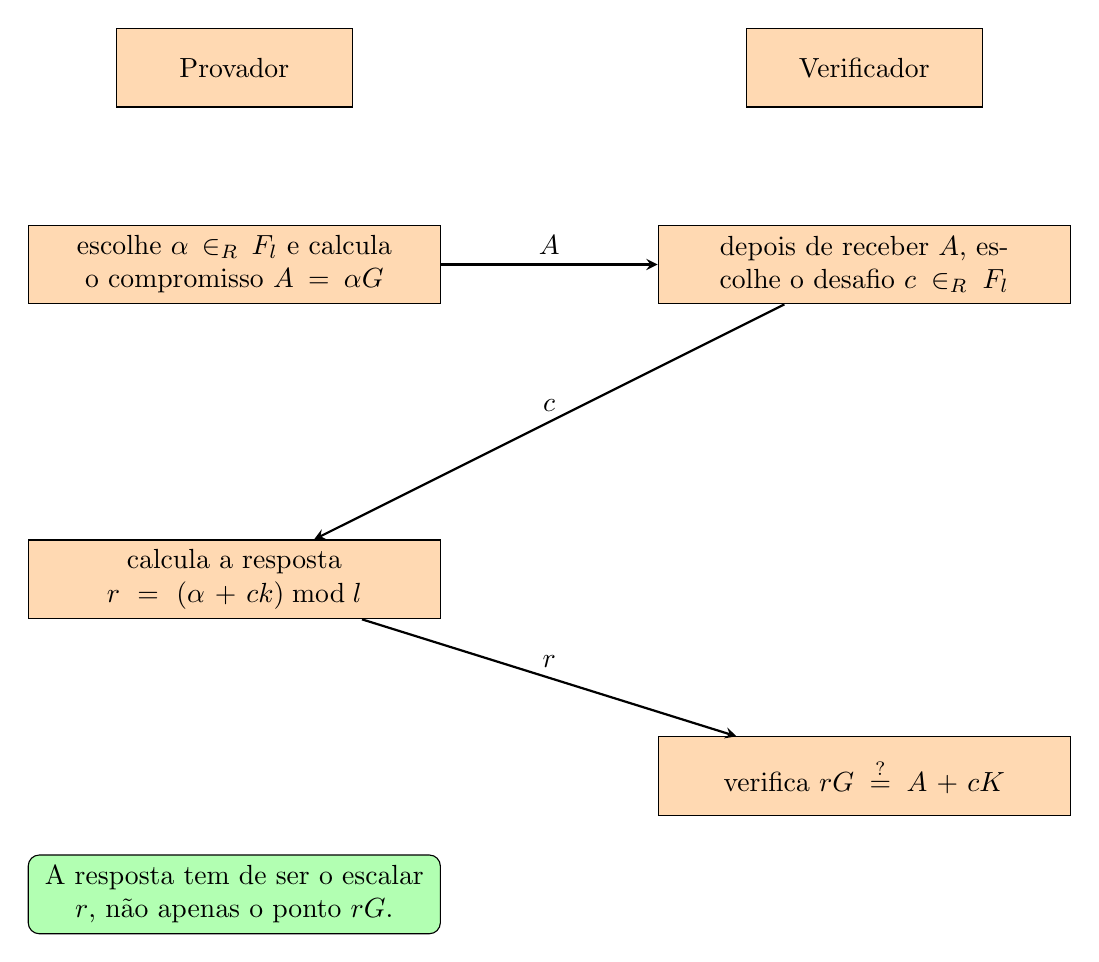
\begin{tikzpicture}[node distance=2cm]
\node (ver0) [process] {Provador};
\node (pro0) [process, right of=ver0, xshift=6cm] {Verificador};
\node (ver1) [process, below of=ver0, yshift=-0.5cm, text width=5cm]
{escolhe \(\alpha\in_R\mathbb{F}_l\) e calcula o compromisso
\(A=\alpha G\)};
\node (pro1) [process, below of=pro0, yshift=-0.5cm, text width=5cm]
{depois de receber \(A\), escolhe o desafio
\(c\in_R\mathbb{F}_l\)};
\node (ver2) [process, below of=ver1, yshift=-2cm, text width=5cm]
{calcula a resposta \(r=(\alpha+ck)\bmod l\)};
\node (pro2) [process, below of=pro1, yshift=-4.5cm, text width=5cm]
{verifica \(rG\stackrel{?}{=}A+cK\)};
\node (ver3) [note, below of=ver2, yshift=-2cm, text width=5cm]
{A resposta tem de ser o escalar \(r\), não apenas o ponto \(rG\).};
%\node (pro2c) [process, right of=pro2a, xshift=8cm] {Process 2b};
%\draw [arrow] (dec1) -- (pro2a);
\draw [arrow] (ver1) -- node[anchor=south] {\(A\)} (pro1);
\draw [arrow] (pro1) -- node[anchor=south] {\(c\)} (ver2);
\draw [arrow] (ver2) -- node[anchor=south] {\(r\)} (pro2);
%\draw [arrow] (pro2b) -- node[anchor=west] {$c$} (pro2c);
\end{tikzpicture}

Um provador honesto é sempre aceite, porque
\[
rG=(\alpha+ck)G=\alpha G+cK=A+cK.
\]
O desafio só é escolhido depois de o compromisso \(A\) ficar fixo. O registo
completo da interacção (o {\em transcript}) contém as três mensagens
\((A,c,r)\); sem \(A\), a equação de verificação nem sequer fica determinada.
Responder apenas com o ponto \(rG\) seria inútil, pois qualquer pessoa poderia
copiar o ponto já calculável \(A+cK\). O trabalho do provador consiste em dar o
seu logaritmo discreto \(r\).

%The verifier can compute $R' = \alpha G + c*K$ before the prover, so providing $c$ is like saying, ``I challenge you to respond with the discrete logarithm of $R'$." A challenge the prover can only overcome by knowing $k$ (except with negligible probability).
Se \(\alpha\) for uniforme, então, para valores fixos de \(c\) e \(k\), a
resposta \(r\) também é uniforme \cite{SCOZZAFAVA1993313}. Mais ainda, no caso
de um verificador que escolhe honestamente um desafio uniforme, podemos simular
um registo sem conhecer \(k\): escolhemos \(c,r\in_R\mathbb{F}_l\) e pomos
\(A=rG-cK\). O resultado tem a mesma distribuição que uma execução real. Esta
é a propriedade de que a interacção não revela informação adicional sobre
\(k\) além da que já estava na chave pública \(K\).
%If $\alpha$ was chosen randomly by the prover then $r$ is randomly distributed \cite{SCOZZAFAVA1993313} and $k$ is information-theoretically secure within $r$ (it can still be found by solving the DLP for $K$ or $\alpha G$).
%\footnote{\label{information_theoretic_note}A cryptosystem with information-theoretic security is one where even an adversary with infinite computing power could not break it, because they simply wouldn't have enough information.} 
Há, porém, uma condição decisiva: o provador não pode reutilizar \(\alpha\).
Se o mesmo compromisso \(A\) receber desafios distintos \(c\ne c'\) e produzir
respostas válidas
\(r=\alpha+ck\) e \(r'=\alpha+c'k\), qualquer observador extrai a chave:
\footnote{Numa prova de segurança, um extractor pode executar o provador duas
vezes a partir do mesmo estado posterior à escolha de \(\alpha\), fornecendo um
desafio diferente em cada execução. Esta técnica é designada por
``rebobinagem'' do provador.}

%However, if the prover reuses $\alpha$ to prove his knowledge of $k$, anyone who knows both challenges in $r = \alpha + c*k$ and $r' = \alpha + c'*k$ can compute $k$ (two equations, two unknowns).
%If the prover is a computer, you could imagine someone `cloning'/copying the computer after it generates $\alpha$, then presenting each copy with a different challenge.}
%In security proofs, phrases like `forking lemma' and `rewind on success' are analagous to this cloning attack. See for example \cite{Liu2004}.
\[
k=(r-r')(c-c')^{-1}\bmod l.
\]
A inversa existe porque \(l\) é primo e \(c-c'\not\equiv0\pmod l\). Esta
possibilidade de extracção explica em que sentido uma resposta válida demonstra
conhecimento, salvo a probabilidade negligível de adivinhar o desafio.

%Se o provador sabia $c$ do início  
%If the prover knew $c$ from the beginning (e.g. if the verifier secretly gave it to her), she could generate a random response $r$ and compute $\alpha G = r G - c K$. When she later sends $r$ to the verifier, she `proves' knowledge of $k$ without ever having to know it. Someone observing the transcript of events between prover and verifier would be none the wiser. The scheme is not {\em publicly verifiable}. \cite{Signatures2015BorromeanRS}\\

O atraso do desafio é essencial. Se conhecesse \(c\) antes de fixar \(A\), um
impostor poderia escolher \(r\) ao acaso e definir \(A=rG-cK\); a verificação
passaria sem que ele conhecesse \(k\). A transformada de Fiat--Shamir
\cite{fiat-shamir-transform} substitui o verificador por uma função hash que só
pode ser avaliada depois de \(A\) estar determinado. No modelo do oráculo
aleatório, isso torna a prova não interactiva e publicamente verificável
\cite{Signatures2015BorromeanRS}.
%In his role as challenger, the verifier spits out a random number after receiving $\alpha G$, making him equivalent to a {\em random function}. Random functions, such as hash functions, are known as random oracles because computing one is like requesting a random number from someone \cite{Signatures2015BorromeanRS}.
\footnote{Em criptografia, um oráculo é uma abstracção que responde a consultas
segundo uma regra especificada. Um oráculo aleatório conserva uma resposta
uniforme e independente para cada entrada nova \cite{cryptographic-oracle}.}
%More generally, ``[i]n cryptography... an oracle is any system which can give some extra information on a system, which otherwise would not be available."\cite{cryptographic-oracle}}
%Using a hash function, instead of the verifier, to generate challenges is known as a {\em Fiat-Shamir transform} \cite{fiat-shamir-transform}, because it makes an interactive proof non-interactive and publicly verifiable \cite{Signatures2015BorromeanRS}.
\footnote{Uma função hash real é determinística. É a análise no modelo do
oráculo aleatório que idealiza cada saída nova como uniforme; a conversão dessa
saída num escalar deve ainda evitar ou limitar o viés de redução.}
%The output of a cryptographic hash function $\mathcal{H}$ is uniformly distributed across the range of possible outputs. That is to say, for some input $A$, $\mathcal{H}(A) \in^D_R \mathbb{S}_H$ where $\mathbb{S}_H$ is the set of possible outputs from $\mathcal{H}$. We use $\in^D_R$ to indicate the function is deterministically random. $\mathcal{H}(A)$ produces the same thing every time, but its output is equivalent to a random number.}
\footnote{O desafio deve ficar ligado à declaração que se prova. Inclui-se a
chave pública \(K\) na hash --- o chamado prefixo de chave --- e, se \(G\) não
for fixo para o protocolo, inclui-se também o gerador. Voltaremos a esta ideia
nas secções \ref{blsag_note} e \ref{sec:robust-key-aggregation}.}
%Note that non-interactive Schnorr-like proofs (and signatures) require either use of a fixed generator $G$, or inclusion of the generator in the challenge hash. Including it that way is known as key prefixing, which we discuss a bit more later (Sections \ref{blsag_note} and \ref{sec:robust-key-aggregation}).}

\subsubsection*{Prova não interactiva}

\iffalse
\begin{enumerate}
	\item Gera-se um número aleatório $\alpha \in_R \mathbb{Z}_l$, e calcula-se $\alpha G$.  
	\item Calcula-se o desafio com uma função hash criptográficamente segura \(c = \mathcal{H}([\alpha G])\).
	\item Define-se a resposta $r = \alpha + c*k$.
	\item Publica-se o par de prova $(\alpha G, r)$.
\end{enumerate}

\subsubsection*{Verificação}

\begin{enumerate}
	\item Calcula-se o desafio: \(c' = \mathcal{H}([\alpha G])\).
	\item Calcula-se $R = r G$ e $R' = \alpha G + c'*K$.
	\item Se $R = R'$ então o provador tem de saber $k$ (enp).
\end{enumerate}
\fi

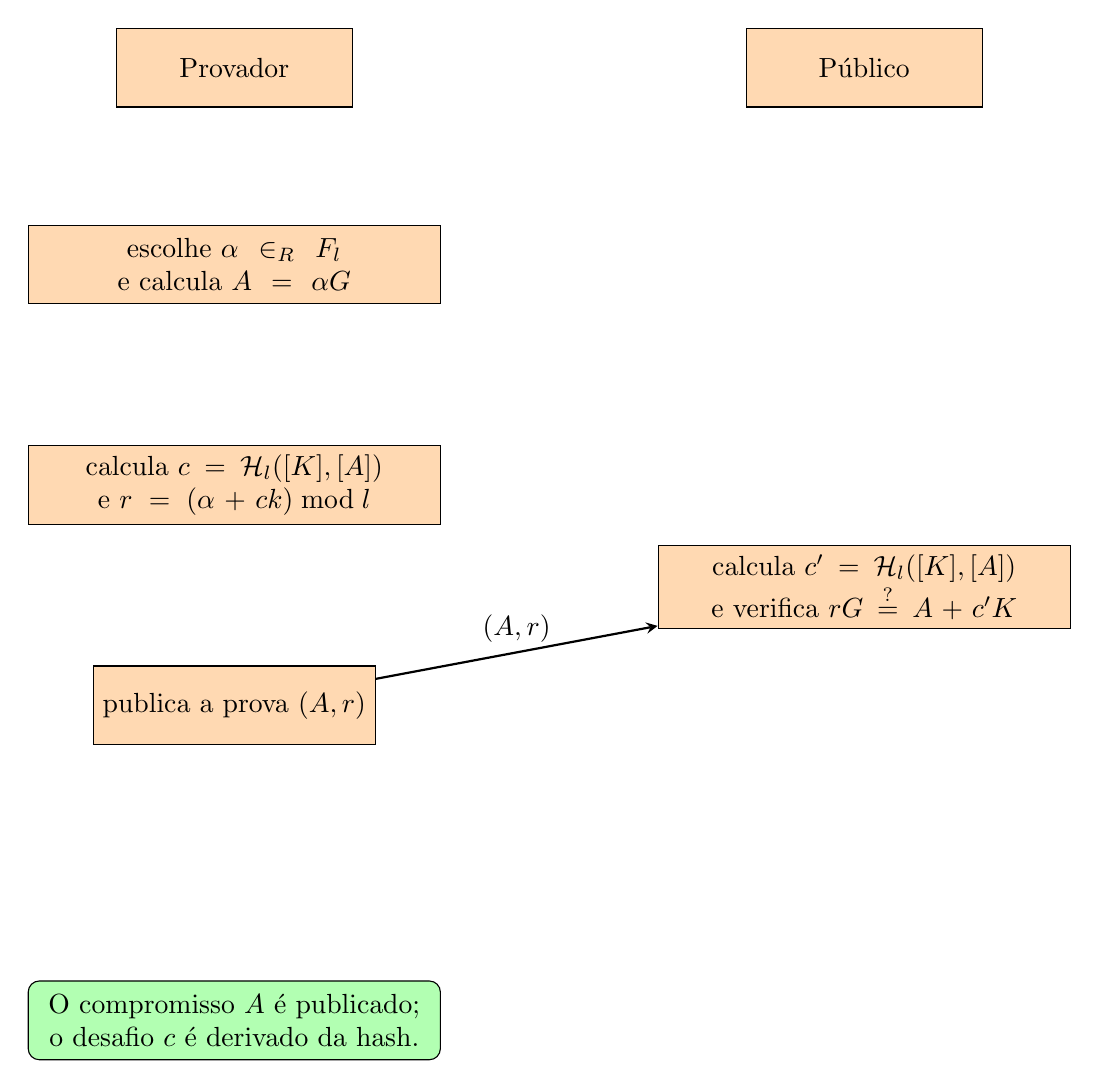
\begin{tikzpicture}[node distance=2cm]
\node (ver0_FS) [process] {Provador};
\node (pro0_FS) [process, right of=ver0_FS, xshift=6cm] {Público};
\node (ver1_FS) [process, below of=ver0_FS, yshift=-0.5cm, text width=5cm]
{escolhe \(\alpha\in_R\mathbb{F}_l\) e calcula \(A=\alpha G\)};
\node (ver2_FS) [process, below of=ver1_FS, yshift=-0.8cm, text width=5cm]
{calcula \(c=\mathcal{H}_l([K],[A])\) e
\(r=(\alpha+ck)\bmod l\)};
\node (ver3_FS) [process, below of=ver2_FS, yshift=-0.8cm]
{publica a prova \((A,r)\)};
\node (pro1_FS) [process, below of=pro0_FS, yshift=-4.6cm, text width=5cm]
{calcula \(c'=\mathcal{H}_l([K],[A])\) e verifica
\(rG\stackrel{?}{=}A+c'K\)};
\node (ver4_FS) [note, below of=ver3_FS, yshift=-2cm, text width=5cm]
{O compromisso \(A\) é publicado; o desafio \(c\) é derivado da hash.};
%\node (pro2c) [process, right of=pro2a, xshift=8cm] {Process 2b};
%\draw [arrow] (dec1) -- (pro2a);
%\draw [arrow] (pro1_FS) -- node[anchor=south] {$c$} (ver2_FS);
\draw [arrow] (ver3_FS) -- node[anchor=south] {\((A,r)\)} (pro1_FS);
%\draw [arrow] (pro2b) -- node[anchor=west] {$c$} (pro2c);
\end{tikzpicture}

Já não há interacção: o provador calcula o desafio localmente e publica uma
única prova. Qualquer pessoa pode repetir a hash e a verificação. A correcção
continua a ser a mesma,
\[
rG=(\alpha+ck)G=A+cK.
\]
É importante distinguir o registo interactivo \((A,c,r)\) da prova
não interactiva publicada \((A,r)\): nesta última, \(c\) é reconstruído de
forma determinística a partir de \(K\) e \(A\).

Os requisitos computacionais de uma prova incluem o espaço necessário para a
guardar e o trabalho de verificação. Neste esquema, a prova contém um ponto de
curva e um escalar; a declaração contém ainda a chave pública, outro ponto. A
verificação exige uma hash e multiplicações escalares da curva.
\marginnote{src/ringct/ rctOps.cpp}


\subsection{Assinar mensagens}
\label{sec:signing-messages}

Um esquema de assinatura recebe uma mensagem de comprimento arbitrário e
incorpora-a numa hash de comprimento fixo. Representaremos por
\(\mathfrak{m}\) a sequência de bytes que o esquema recebe. Algumas variantes
definem uma modalidade de pré-hash, na qual essa entrada já é a hash da mensagem;
essa escolha faz parte do protocolo e não deve ficar implícita.

%Typically, a cryptographic signature is performed on a cryptographic hash of a message rather than the message itself, which facilitates signing messages of varying size. However, in this report we will loosely use the term `message', and its symbol $\mathfrak{m}$, to refer to the message properly speaking and/or its hash value, unless specified.
As assinaturas permitem ao destinatário verificar que uma mensagem foi
autorizada pelo titular de uma chave privada e que o conteúdo assinado não foi
alterado. ECDSA é um esquema comum; veja-se \cite{ecdsa}, ANSI X9.62 e
\cite{Hankerson:2003:GEC:940321}.

%Signing messages is a staple of Internet security that lets a message's recipient be confident its content is as intended by the signer. One common signature scheme is called ECDSA. See \cite{ecdsa}, ANSI X9.62, and \cite{Hankerson:2003:GEC:940321}.

O esquema seguinte é uma formulação da prova de Schnorr transformada, com uma
convenção de sinais que permite publicar dois escalares \((c,r)\) em vez do
ponto \(A\). Pensar em assinaturas desta forma preparar-nos-á para as
assinaturas em anel do capítulo seguinte.

%The signature scheme we present here is an alternative formulation of the transformed Schnorr proof from before. Thinking of signatures in this way prepares us for exploring ring signatures in the next chapter.

\iffalse

\subsubsection*{Assinatura}

Seja que a alice tem um par de chaves \((k_A, K_A)\). Para unequivocamente assinar uma mensagem arbitrária $\mathfrak{m}$, os seguintes passos são executados :

%Assume Alice has the private/public key pair \((k_A, K_A)\). To unequivocally sign an arbitrary message $\mathfrak{m}$, she could execute the following steps:

\begin{enumerate}
	\item Generate random number $\alpha \in_R \mathbb{Z}_l$, and compute $\alpha G$.
	\item Calculate the challenge using a cryptographically secure hash function, \(c = \mathcal{H}(\mathfrak{m},[\alpha G])\).
	\item Define the response $r$ such that $\alpha = r + c*k_A$. In other words, $r = \alpha - c*k_A$.
	\item Publish the signature $(c, r)$.
\end{enumerate}

\subsubsection*{Verificação}

Qualquer entidade terceira que saiba os parametros de CE, a assinatura $(c, r)$ e o methodo de assinatura, a mensagem $\mathfrak{m}$, a função hash e $K_A$ pode verificar a assinatura :

%Any third party who knows the EC domain parameters (specifying which elliptic curve was used), the signature $(c, r)$ and the signing method, $\mathfrak{m}$ and the hash function, and $K_A$ can verify the signature:

\begin{enumerate}
	\item Calcula-se o desafio: \(c' = \mathcal{H}(\mathfrak{m},[r G + c*K_A])\).
	\item Se $c = c'$ então a assinatura é válida.
\end{enumerate}

\fi

Alice tem o par \((k_A,K_A)\). Para cada mensagem, escolhe um escalar secreto
\(\alpha\) novo e imprevisível; reutilizá-lo exporia \(k_A\), exactamente como
na prova interactiva.

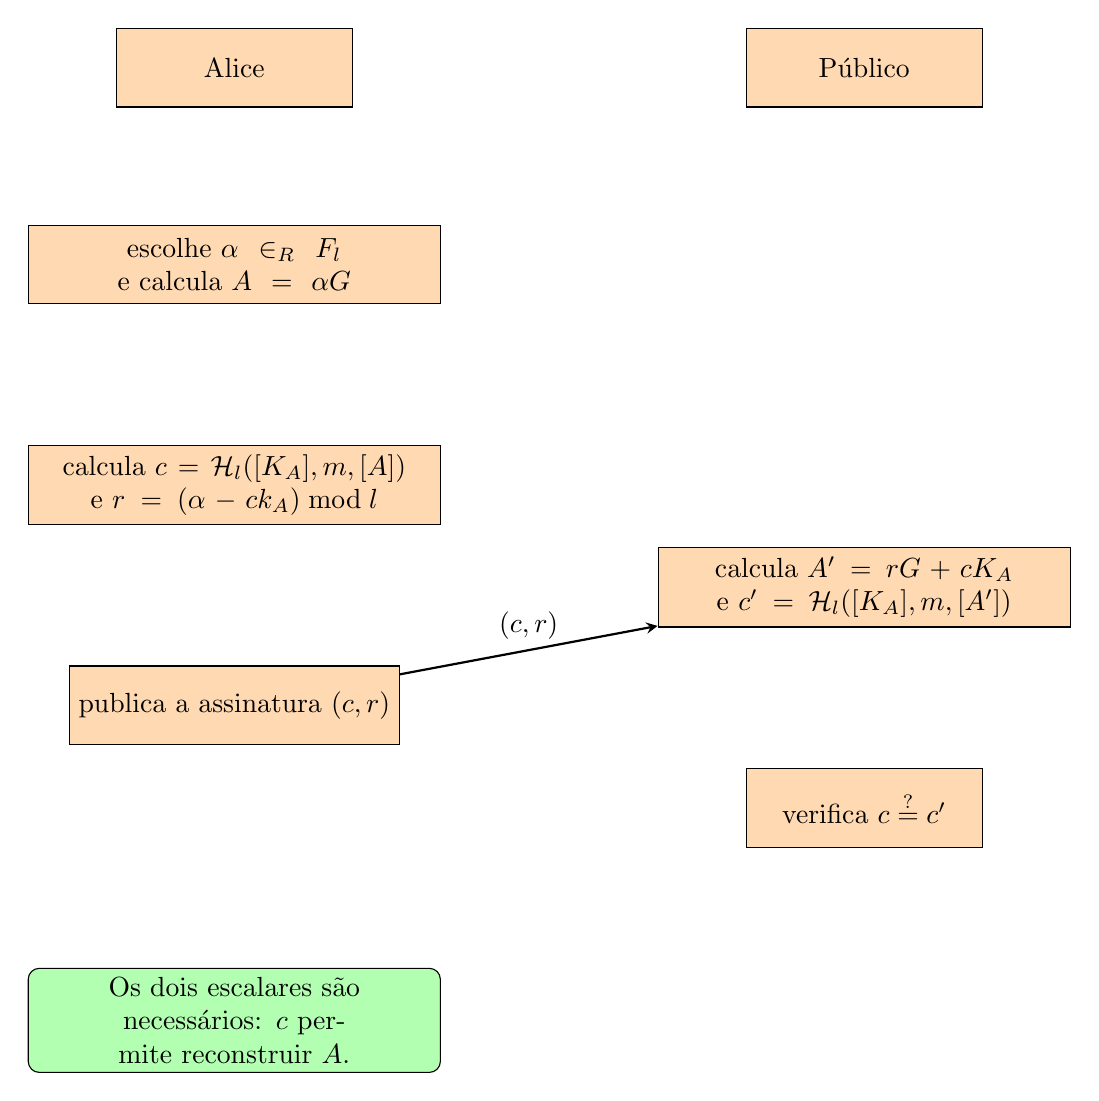
\begin{tikzpicture}[node distance=2cm]
\node (ver0_SM) [process] {Alice};
\node (pro0_SM) [process, right of=ver0_SM, xshift=6cm] {Público};
\node (ver1_SM) [process, below of=ver0_SM, yshift=-0.5cm, text width=5cm]
{escolhe \(\alpha\in_R\mathbb{F}_l\) e calcula \(A=\alpha G\)};
\node (ver2_SM) [process, below of=ver1_SM, yshift=-0.8cm, text width=5cm]
{calcula \(c=\mathcal{H}_l([K_A],\mathfrak{m},[A])\) e
\(r=(\alpha-ck_A)\bmod l\)};
\node (ver3_SM) [process, below of=ver2_SM, yshift=-0.8cm]
{publica a assinatura \((c,r)\)};
\node (ver4_SM) [note, below of=ver3_SM, yshift=-2cm, text width=5cm]
{Os dois escalares são necessários: \(c\) permite reconstruir \(A\).};
%\node (pro2_SM) [process, below of=pro1_SM, yshift=-0.5cm, text width=4.5cm] {
%\(     r G &= (\alpha - c*k_A) G \\
%  	  	 &= \alpha G - c*K_A, então :    
%     \alpha G &= r G + c*K_A    \)
%};
\node (pro1_SM) [process, below of=pro0_SM, yshift=-4.6cm, text width=5cm]
{calcula \(A'=rG+cK_A\) e
\(c'=\mathcal{H}_l([K_A],\mathfrak{m},[A'])\)};
\node (pro4_SM) [process, below of=pro1_SM, yshift=-0.8cm]
{verifica \(c\stackrel{?}{=}c'\)};
%\node (pro2c) [process, right of=pro2a, xshift=8cm] {Process 2b};
%\draw [arrow] (dec1) -- (pro2a);
%\draw [arrow] (pro1_FS) -- node[anchor=south] {$c$} (ver2_FS);
\draw [arrow] (ver3_SM) -- node[anchor=south] {\((c,r)\)} (pro1_SM);
%\draw [arrow] (pro2b) -- node[anchor=west] {$c$} (pro2c);
\end{tikzpicture}

Se \(c=c'\), a assinatura é válida. A chave pública e a mensagem entram na
hash, e as codificações devem ser inequívocas; um protocolo real inclui ainda
um separador de domínio para não reutilizar o mesmo desafio noutro contexto.
  
%In this signature scheme we store two scalars, and need one public EC key.

\subsubsection*{Funciona porque}

O verificador reconstrói exactamente o compromisso de Alice:
%This stems from the fact that
\begin{align*}
r&=\alpha-ck_A,\\
A'&=rG+cK_A\\
  &=(\alpha-ck_A)G+cK_A\\
  &=\alpha G-cK_A+cK_A\\
  &=\alpha G=A.
\end{align*}
Logo,
\[
c'=\mathcal{H}_l([K_A],\mathfrak{m},[A'])
  =\mathcal{H}_l([K_A],\mathfrak{m},[A])=c.
\]

Portanto, uma assinatura produzida por Alice passa a verificação. Esta álgebra
demonstra a correcção, não basta por si só para provar a infalsificabilidade;
essa propriedade depende da dificuldade do PLD, da segurança da hash, da
escolha correcta de \(\alpha\) e do modelo de segurança do esquema.


Requisitos:

Neste esquema, a assinatura guarda dois escalares. Para a verificar, são ainda
necessários a mensagem, a chave pública de curva e os parâmetros do protocolo.

%Therefore the owner of $k_A$ (Alice) created $(c,r)$ for $\mathfrak{m}$: she signed the message. The probability someone else, a forger without $k_A$, could have made $(c,r)$ is negligible, so a verifier can be confident the message was not tampered with.



%----------CURVE ED25519
\section{Curva Edwards25519}
\label{Ed25519_section}

Monero usa a curva de Edwards torcida {\em Edwards25519}, que é birracionalmente
equivalente à curva de Montgomery {\em Curve25519}.
%Monero uses a particular Twisted Edwards elliptic curve for cryptographic operations, {\em Ed25519}, the {\em birational equivalent}
\footnote{\label{birational_note}Sem entrarmos nos pormenores, uma equivalência
birracional relaciona pontos das duas curvas por funções racionais, com as
excepções que essas funções necessariamente admitem.}
%Without giving further details, birational equivalence can be thought of as an isomorphism expressible using rational terms.} 
%of the Montgomery curve {\em Curve25519}.
As construções Curve25519, Edwards25519 e Ed25519 foram publicadas por
Bernstein e colaboradores
\cite{curve25519,Bernstein2008,Bernstein2012,Bernstein2007}.
Convém não confundir os nomes: Edwards25519 é a curva; Ed25519 é uma instância
do esquema de assinatura EdDSA sobre essa curva, que estudaremos mais abaixo.
%Both Curve25519 and Ed25519 were released by Bernstein {\em et al.} \cite{Bernstein2008, Bernstein2012, Bernstein2007}.
\footnote{Bernstein desenvolveu também a cifra ChaCha
\cite{Bernstein_chacha,chacha-irtf}, usada pela implementação Monero
\cite{monero-source-v16} para cifrar\marginnote{src/wallet/ ringdb.cpp} certos
dados sensíveis da carteira.}

%also developed an encryption scheme known as ChaCha \cite{Bernstein_chacha,chacha-irtf}, which the primary Monero implementation uses to encrypt\marginnote{src/wallet/ ringdb.cpp} certain sensitive information related to users' wallets.}

A curva é definida sobre o corpo primo \(\mathbb{F}_q\), com
\(q=2^{255}-19\), pela equação
%The
\marginnote{src/crypto/ crypto\_ops\_ builder/ ref10Comm- entedComb- ined/\\ ge.h} %curve is defined over the prime field \(\mathbb{F}_{2^{255} - 19}\) (i.e. $q = 2^{255}-19$) by means of the following equation:
\[
-x^2+y^2=1-\frac{121665}{121666}x^2y^2.
\]
A fracção representa uma divisão em \(\mathbb{F}_q\). Assim, na notação geral
da secção \ref{elliptic_curves_section}, \(a=-1\) e
\(d=-121665/121666\bmod q\).

Os parâmetros foram escolhidos por um processo público e explicável. Essa
propriedade, por vezes chamada rigidez, reduz a liberdade que um criador teria
para procurar secretamente uma curva com uma fraqueza rara.
%This curve addresses many concerns raised by the cryptography community.
\footnote{Uma curva pode não ter fraquezas públicas conhecidas e, ainda assim,
ter sido seleccionada entre muitas candidatas por uma razão que o seu criador
não revelou. Exigir uma derivação reproduzível dos parâmetros limita esse
espaço de escolha. Edwards25519 é classificada como uma curva de geração
totalmente explicada \cite{elliptic-curve-rigidity}.}

%Even if a curve appears to have no cryptographic security problems, it's possible the person/organization that created it knows a secret issue that only crops up in very rare curves. Such a person may have to randomly generate many curves in order to find one with a hidden weakness and no known weaknesses. If reasonable explanations are required for curve parameters, then it becomes even more difficult to find weak curves that will be accepted by the cryptographic community. Curve Ed25519 is known as a `fully rigid' curve, which means its generation process was fully explained. \cite{elliptic-curve-rigidity}} 
O cuidado não é apenas teórico. O gerador Dual\_EC\_DRBG, que chegou a ser
normalizado pelo NIST\footnote{\label{NIST_note}National Institute of Standards
and Technology, \url{https://www.nist.gov/}}, ficou associado a um potencial
mecanismo secreto de exploração baseado nos seus parâmetros elípticos
\cite{hales2014nsa}. A
influência da NSA sobre esse processo de normalização tornou-se um exemplo dos
riscos de concentrar escolhas criptográficas pouco transparentes
\cite{NSA-NIST}. Isto não implica que todos os standards do NIST sejam
defeituosos; explica por que valorizamos parâmetros reproduzíveis e diversidade
de análise.
%It is well known that NIST
%\footnote{\label{NIST_note}National Institute of Standards and Technology, \url{https://www.nist.gov/}} 
%standard algorithms have issues. For example, it has recently become clear the NIST standard random number generation algorithm PNRG (the version based on elliptic curves) is flawed and contains a potential backdoor \cite{hales2014nsa}. Seen from a broader perspective, standardization authorities like NIST lead to a cryptographic monoculture, introducing a point of centralization. A great example of this was illustrated when the NSA used its influence over NIST to weaken an international cryptographic standard \cite{NSA-NIST}.
O projecto Edwards25519 foi também apresentado com atenção à ausência de
restrições por patentes (veja-se \cite{ECC-patents}) e a operações eficientes
\marginnote{src/crypto/ crypto\_ops\_ builder/} \cite{Bernstein2007}.
%Curve Ed25519 is not subject to any patents (see \cite{ECC-patents} for a discussion on this subject), and the team behind it has
%developed\marginnote{src/crypto/ crypto\_ops\_ builder/} and adapted basic cryptographic algorithms with efficiency in mind \cite{Bernstein2007}.
O grupo de pontos de Edwards25519 tem ordem \(N=hl\), com cofactor
\(h=8=2^3\) e ordem prima
%Twisted Edwards curves have order expressible as \(N=2^c l\), where \(l\) is a prime number and \(c\) a positive integer. In the case of curve Ed25519, its order is a 76 digit number ($l$ is 253 bits):
\[
l=72370055773322622139731865630429942408\,
57116359379907606001950938285454250989.
\]
\marginnote{src/ringct/ rctOps.h {\tt curve- Order()}}
O inteiro \(l\) tem comprimento binário de 253 bits, pois
\(2^{252}<l<2^{253}\); isso não significa que um escalar uniforme contenha
253 bits completos de entropia. A sua entropia é \(\log_2 l\), muito próxima
de 252 bits. Escalares e chaves privadas são habitualmente guardados em
recipientes de 32 bytes, mas o tamanho da representação, o comprimento binário
do módulo e a entropia são três grandezas distintas. A ordem total \(8l\), por
sua vez, é um inteiro de 256 bits e tem 77 algarismos decimais.


\subsection{Representação binária}
\label{binary_note}
O representante canónico de um elemento de
\(\mathbb{F}_{2^{255}-19}\) está entre \(0\) e \(q-1\), pelo que cabe em 255
bits. A codificação usada por Edwards25519 ocupa 32 bytes em ordem
{\em little-endian}; antes da compressão de pontos, o bit 255 desse recipiente
está livre. Duas coordenadas completas ocupariam, portanto, 64 bytes.

Um escalar canónico em \(\mathbb{F}_l\) também é guardado em 32 bytes, mas
obedece ao limite diferente \(0\leq s<l\). Não devemos confundir uma sequência
arbitrária de 32 bytes, um elemento do corpo de coordenadas, um escalar reduzido
e uma codificação canónica: têm o mesmo tamanho exterior, não o mesmo domínio.
%Elements of \(\mathbb{F}_{2^{255} - 19} \) are encoded as 256-bit integers, so they can be represented using 32 bytes. Since each element only requires 255 bits, the most significant bit is always zero.

%Consequently, any point in Ed25519 could be expressed using 64 bytes. By applying {\em point compression} techniques, described here below, however, it is possible to reduce this amount by half, to 32 bytes.

\subsection{Compressão de ponto elíptico}
\label{point_compression_section}

Um ponto de Edwards25519 pode ser codificado nos mesmos 32 bytes que uma única
coordenada. A ideia geral de compressão de pontos é anterior a esta curva
\cite{Miller:point-compression-origin}; a codificação de Edwards25519 é descrita
em \cite{Bernstein2012,eddsa-ed25519-irtf}.

%The Ed25519 curve has the property that its points can be easily compressed, so that representing a point will consume only the space of one coordinate. We will not delve into the mathematics necessary to justify this, but we can give a brief insight into how it works \cite{eddsa-ed25519-irtf}. Point compression for the Ed25519 curve was first described in \cite{Bernstein2012}, while the concept was first introduced in \cite{Miller:point-compression-origin}.

Com \(a=-1\), a equação da curva pode ser reorganizada como
\[
x^2=\frac{y^2-1}{dy^2+1},
\qquad d=-\frac{121665}{121666}\bmod q.
\]
Para um \(y\) válido, recuperar \(x\) consiste em extrair uma raiz quadrada no
corpo. Em regra há duas possibilidades, \(x\) e \(-x\); quando \(x=0\), elas
coincidem. Como \(q\) é ímpar, os representantes canónicos de \(x\ne0\) e
\(-x\) têm paridades opostas: por exemplo, módulo \(5\), os valores \(3\) e
\(-3\bmod5=2\) são um ímpar e um par. Um único bit escolhe, portanto, a raiz
pretendida.
%This point compression scheme follows from a transformation of the Twisted Edwards curve equation (assuming $a = -1$, which is true for Monero): $x^2 = (y^2-1)/(d y^2+1)$,
%\footnote{Here $d = - \frac{121665}{121666}$.} 
%which indicates there are two possible $x$ values ($+$ or $-$) for each $y$. Field elements $x$ and $y$ are calculated$\pmod{q}$, so there are no actual negative values. However, taking$\pmod{q}$ of $–x$ will change the value between odd and even since $q$ is odd. For example: $3 \pmod{5} = 3$, $-3 \pmod{5} = 2$. In other words, the field elements $x$ and $–x$ have different odd/even assignments.
Esse bit cabe na posição 255, que estava livre na codificação de \(y\). Eis o
procedimento conceptual para um ponto \((x,y)\):


%If we have a curve point and know its $x$ is even, but given its $y$ value the transformed curve equation outputs an odd number, then we know negating that number will give us the right $x$. One bit can convey this information, and conveniently the $y$ coordinate has an extra bit.

%Assume we want to compress a point \((x, y)\).

\begin{description}
	\item[Codificar] Codifica-se \(y\) canonicamente em 32 bytes
    {\em little-endian}\marginnote{src/crypto/ crypto\_ops\_ builder/
    ref10Comm- entedComb- ined/\\ ge\_to- bytes.c} e coloca-se no bit 255 a
    paridade do representante canónico de \(x\): zero se \(x\) é par, um se é
    ímpar. Chamemos \(y'\) ao resultado.
%We\marginnote{src/crypto/ crypto\_ops\_ builder/ ref10Comm- entedComb- ined/\\ ge\_to- bytes.c} set the most significant bit of $y$ to 0 if $x$ is even, and 1 if it is odd. The resulting value $y’$ will represent the curve point.
	
	\item[Descodificar] \hfill
	    \begin{enumerate}
            \item Copie-se o bit 255 de \(y'\) para \(b\), limpe-se esse bit e
            interpretem-se os restantes como \(y\). Rejeita-se a codificação
            se \(y\geq q\), pois não seria canónica.
            \marginnote{ge\_from- bytes.c}[2.05cm]
%Retrieve\marginnote{ge\_from- bytes.c}[2.05cm] the compressed point $y’$, then copy its most significant bit to the parity bit $b$ before setting it to 0. Now it is the original $y$ again.
            \item Calcule-se \(u=(y^2-1)\bmod q\) e
            \(v=(dy^2+1)\bmod q\), de modo que \(x^2=u/v\) no corpo.
            \item Calcule-se\footnote{Como
            \(q=2^{255}-19\equiv5\pmod8\), os expoentes \((q-5)/8\) e
            \((q-1)/4\) são inteiros.}
            \[
            z=uv^3(uv^7)^{(q-5)/8}\bmod q.
            \]
            \begin{enumerate}
                \item Se \(vz^2\equiv u\pmod q\), ponha-se \(x'=z\).
                \item Se \(vz^2\equiv-u\pmod q\), ponha-se
                \(x'=z\,2^{(q-1)/4}\bmod q\).
                \item Se nenhuma congruência se verificar, \(y'\) não codifica
                um ponto e deve ser rejeitado.
            \end{enumerate}
            \item Se a paridade de \(x'\) diferir de \(b\), ponha-se
            \(x=(-x')\bmod q\); caso contrário, \(x=x'\). Rejeita-se ainda o
            caso \(x=0\) e \(b=1\), a codificação não canónica de ``zero
            negativo''.
%Using the parity bit \(b\) from the first step, if $b \ne$ the least significant bit of $x'$ then  \(x = -x' \pmod q\), otherwise \(x = x'\).
            \item O resultado é o ponto descomprimido \((x,y)\).
%Return the decompressed point $(x,y)$.
	    \end{enumerate}
\end{description}

O gerador convencional do subgrupo de ordem \(l\) é
\(G=(x,4/5)\), com a raiz par de \(x\) \cite{Bernstein2012}. Por isso, a sua
codificação usa \(y=4/5\bmod q\) e bit de sinal zero.

%Implementations of Ed25519 (such as Monero) typically use the generator $G = (x,4/5)$ \cite{Bernstein2012}, where x is the `even', or $b = 0$, variant based on point decompression of \(y = 4/5 \pmod q\).

\subsection{Algoritmo de assinatura EdDSA}
\label{EdDSA_section}

%Bernstein and his team have developed a number of basic algorithms based on curve Ed25519.\footnote{\label{group_ops_twisted_edwards_note}See\marginnote{src/crypto/ crypto\_ops\_ builder/ ref10Comm- entedComb- ined/} \cite{Bernstein2007} for efficient group operations in Twisted Edwards EC (i.e. point addition, doubling, mixed addition, etc). See \cite{curve25519} for efficient modular arithmetic.}
%!!!2
EdDSA designa uma família de assinaturas de estilo Schnorr. {\em Ed25519} é a
instância que usa Edwards25519; não é o nome da curva. O artigo original
apresentou-a como uma alternativa eficiente a ECDSA e relatou mais de 100~000
assinaturas por segundo no equipamento então usado \cite{Bernstein2012}. A
especificação completa encontra-se na RFC 8032 \cite{rfc8032}.
%For illustration purposes we will describe a highly optimized and secure alternative to the ECDSA signature scheme which, according to the authors, allows producing over 100 000 signatures per second using a commodity Intel Xeon processor \cite{Bernstein2012}. The algorithm can also be found described in Internet RFC8032 \cite{rfc8032}. Note this is a very Schnorr-like signature scheme.
Ed25519 deriva o valor efémero deterministicamente de um segredo e da mensagem,
em vez de pedir ao sistema um novo número aleatório por assinatura. Isto evita
uma classe importante de falhas de geradores aleatórios, embora não elimine a
necessidade de proteger o segredo, a implementação e os cálculos contra falhas
e canais laterais. O desenho procura, entre outros objectivos, evitar acessos a
posições de memória dependentes de dados secretos e reduzir ataques temporais à
cache \cite{Bernstein2012}.

A chave privada externa é uma semente \(s\) de 32 bytes. Ed25519 calcula uma
hash SHA-512 dessa semente. Os primeiros 32 bytes são podados: limpam-se os
três bits menos significativos e o bit mais significativo, e fixa-se o segundo
bit mais significativo. Interpretado em {\em little-endian}, o resultado é o
inteiro secreto \(a\); os 32 bytes restantes formam um prefixo secreto \(p\).
A chave pública é \(A=aG\), transmitida na sua codificação comprimida \([A]\).

Estas grandezas voltam a ilustrar a diferença entre tamanho e entropia. Uma
semente uniforme de 32 bytes tem 256 bits de entropia; o inteiro podado \(a\)
tem comprimento de 255 bits, mas apenas 251 posições variáveis, e não é uma
codificação canónica de um escalar menor que \(l\). Já os escalares da
assinatura são reduzidos módulo \(l\) e codificados em 32 bytes.

%Among other things, instead of generating random integers every time, it uses a hash value derived from the private key of the signer and the message itself. This circumvents security flaws related to the implementation of random number generators. Also, another goal of the algorithm is to avoid accessing secret or unpredictable memory locations to prevent so-called {\em cache timing attacks} \cite{Bernstein2012}.
%We provide here an outline of the steps performed by the algorithm. A complete description and sample implementation in the Python language can be found in \cite{rfc8032}. 

\subsubsection*{Assinatura}

Para a variante pura Ed25519, seja \(\mathfrak{m}\) a mensagem exacta. A
variante Ed25519ph, que recebe uma pré-hash, é um protocolo distinto e tem de
ser seleccionada explicitamente \cite{rfc8032}. Escrevendo \(\mathcal{H}_l\)
para SHA-512 seguida da conversão e redução módulo \(l\):

\begin{enumerate}
	\item Calcule-se o escalar efémero
    \(\rho=\mathcal{H}_l(p,\mathfrak{m})\) e o ponto \(R=\rho G\).

%Let \(h_k\) be a hash \(\mathcal{H}(k)\) of the signer's private key \(k\). Compute \(\alpha\) as a hash \(\alpha = \mathcal{H}(h_k, \mathfrak{m})\) of the hashed private key and message. Depending on implementation, $\mathfrak{m}$ could be the actual message or its hash \cite{rfc8032}.
	
	\item Calcule-se o desafio
    \(e=\mathcal{H}_l([R],[A],\mathfrak{m})\).

	\item Calcule-se \(S=(\rho+ea)\bmod l\).
	
	\item A assinatura é \(([R],[S])\), um ponto comprimido e um escalar
    canónico.
\end{enumerate}

\subsubsection*{Verificação}
A verificação procede da seguinte forma:

\begin{enumerate}
	\item Descodifiquem-se \([A]\) e \([R]\) como pontos e \([S]\) como
    escalar. Rejeitem-se codificações inválidas ou não canónicas e valores
    \(S\geq l\).
	\item Calcule-se \(e'=\mathcal{H}_l([R],[A],\mathfrak{m})\).
	\item Aceite-se apenas se a equação de verificação da RFC 8032 se cumprir:
    \[
    8SG\stackrel{?}{=}8R+8e'A.
    \]
\end{enumerate}

O factor \(8=2^3\) é o cofactor de Edwards25519
\cite{Bernstein2012,rfc8032}. Multiplicar um ponto arbitrário por \(8\) elimina
a sua componente de pequena ordem; não demonstra que o ponto original já
pertencia ao subgrupo primo. Em particular, a equação cofactorizada compara os
dois lados depois de apagar possíveis componentes de torção.
%The $2^c$ term comes from Bernstein {\em et al.}’s general form of the EdDSA algorithm \cite{Bernstein2012}. According to that paper, though it isn’t required for adequate verification, removing $2^c$ provides stronger equations.
Uma verificação explícita \(lA\stackrel{?}{=}0\), acompanhada da rejeição da
identidade, testa se a chave pública pertence ao subgrupo de ordem \(l\). Não é
sinónima de multiplicar toda a equação pelo cofactor. Protocolos e bibliotecas
podem escolher regras de validação mais estritas, mas signatário e verificador
têm de concordar exactamente nas mesmas regras. Esta distinção reaparecerá na
secção \ref{blsag_note}.

%The public key $K$ can be any EC point, but we only want to use points in the generator $G$'s subgroup. Multiplying by the cofactor $2^c$ ensures all points are in that subgroup. Alternatively, verifiers could check $l K \stackrel{?}{=} 0$, which only works if $K$ is in the subgroup. We do not know of any weaknesses caught by these precautions, though as we will see the latter method is important in Monero (Section \ref{blsag_note}).


\subsubsection*{Funciona porque}

Para uma assinatura honesta, \(A=aG\) e \(R=\rho G\). Logo,
\begin{align*}
8SG&=8(\rho+ea)G\\
   &=8\rho G+8e(aG)\\
   &=8R+8eA.
\end{align*}
O verificador recompõe o mesmo \(e\) a partir da mensagem, da chave e de
\([R]\), pelo que a igualdade se verifica.


%By default, an EdDSA signature would need \(64 + 32\) bytes for the EC point $\alpha G$ and scalar $r$. However, RFC8032 assumes point \(\alpha G\) is compressed, which reduces space requirements to only \(32 + 32\) bytes. We include the public key $K$, which implies \(32 + 32 + 32\) total bytes.

Requisitos:

A assinatura Ed25519 guarda um ponto comprimido de 32 bytes e um escalar de 32
bytes: 64 bytes no total. A chave pública comprimida ocupa mais 32 bytes, mas
normalmente é fornecida separadamente da assinatura. A semente privada nunca é
transmitida.

\section{Operador binário XOR}
\label{sec:XOR_section}

O operador binário XOR será útil nas secções \ref{sec:integrated-addresses} e
\ref{sec:pedersen_monero}.
%The binary operator XOR is a useful tool that will appear in Sections \ref{sec:integrated-addresses} and \ref{sec:pedersen_monero}. 
Recebe dois bits e devolve \(1\) se exactamente um deles for \(1\)
%It takes two arguments and returns true if one, but not both, of them is true 
\cite{wolfram-xor}. Eis a tabela de verdade:

\begin{center}
    \begin{tabular}{|c|c|c|}
    \hline
        A & B & A \(\oplus\) B \\
    \hline\hline
        1 & 1 & 0 \\
    \hline
        1 & 0 & 1 \\
    \hline
        0 & 1 & 1 \\
    \hline
        0 & 0 & 0 \\
    \hline
    \end{tabular}
\end{center}

Bit a bit, XOR é a adição módulo \(2\). Por exemplo,
%In the context of computer science, XOR is equivalent to bit addition modulo 2. For example, the XOR of two bit pairs:
\[
\{1,1\}\oplus\{1,0\}
=\{(1+1)\bmod2,(1+0)\bmod2\}
=\{0,1\}.
\]
Da tabela seguem três identidades simples:
\[
A\oplus0=A,\qquad A\oplus A=0,\qquad
(A\oplus B)\oplus B=A.
\]

%Each of these also produce $\{0,1\}$: $\text{XOR}(\{1,0\},\{1,1\})$, $\text{XOR}(\{0,0\},\{0,1\})$, and $\text{XOR}(\{0,1\},\{0,0\})$. 
%For XOR inputs with $b$ bits, there are $2^{\text{b}} - 1$ other combinations of inputs that would make the same output. This means if $C = \text{XOR}(A,B)$ and input $A \in_R \{0,...,2^{\text{b}-1}\}$, an observer who learned $C$ would gain no information about $B$.

%At the same time, anyone who knows two of the elements in $\{A,B,C\}$, where $C = \text{XOR}(A,B)$, can calculate the third element, such as $A = \text{XOR}(B,C)$. XOR indicates if two elements are different or the same, so knowing $C$ and $B$ is enough to expose $A$. A careful examination of the truth table reveals this vital feature.
Suponhamos que Alice quer cifrar um vector privado \(V\) de \(n\) bits. Ela
escolhe uma chave \(S\) também de \(n\) bits e envia a Bob
\[
C=V\oplus S.
\]
Bob, que conhece \(S\), recupera a mensagem porque
\[
C\oplus S=(V\oplus S)\oplus S=V.
\]
Para cada valor fixo de \(C\), há \(2^n\) pares \((V,S)\) que o produzem: a
cada candidato \(V\) corresponde exactamente \(S=C\oplus V\).
\footnote{Outra aplicação de XOR é trocar dois registos sem um terceiro:
\(\{A,B\}\rightarrow\{A\oplus B,B\}\rightarrow
\{A\oplus B,A\}\rightarrow\{B,A\}\).}

\tikzstyle{process} = [rectangle, minimum width=3cm, minimum height=1cm, text centered, draw=black, fill=orange!30]
\tikzstyle{arrow} = [thick,->,>=stealth]
\bigskip
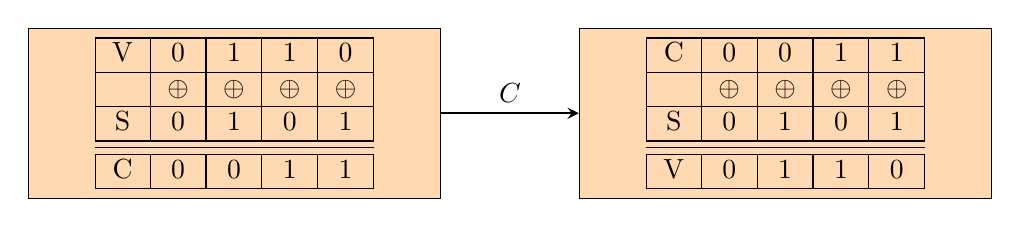
\begin{tikzpicture}[node distance=2cm]
\node (sig0_XOR) [process, text width=5cm] 
{
\begin{tabular}{|c|c|c|c|c|}
    \hline
        V & 0 & 1 & 1 & 0 \\
    \hline
        & $\oplus$ & $\oplus$ & $\oplus$ & $\oplus$ \\
    \hline
        S & 0 & 1 & 0 & 1 \\ 
    \hline\hline\hline
        C & 0 & 0 & 1 & 1 \\
    \hline
\end{tabular}
};
\node (ver0_XOR) [process, right of=sig0_XOR, xshift=5cm, text width=5cm] 
{
\begin{tabular}{|c|c|c|c|c|}
    \hline
        C & 0 & 0 & 1 & 1 \\
    \hline
        & $\oplus$ & $\oplus$ & $\oplus$ & $\oplus$ \\
    \hline
        S & 0 & 1 & 0 & 1 \\
    \hline\hline\hline
        V & 0 & 1 & 1 & 0 \\
    \hline
\end{tabular}
};
%\node (pro2c) [process, right of=pro2a, xshift=8cm] {Process 2b};
%\draw [arrow] (dec1) -- (pro2a);
\draw [arrow] (sig0_XOR) -- node[anchor=south] {$C$} (ver0_XOR);
\end{tikzpicture}

Isto só dá segredo perfeito, no sentido da teoria da informação, sob hipóteses
fortes: \(S\) tem de ser secreta, uniforme em \(\{0,1\}^n\), independente de
\(V\) e usada uma única vez. Nessas condições, observar \(C\) não altera a
probabilidade de qualquer mensagem. Se a mesma chave for reutilizada, então
\(C_1\oplus C_2=V_1\oplus V_2\), o que revela uma relação entre as mensagens.
Uma chave enviesada, previsível ou mais curta também destrói a conclusão.

Quando \(S\) é derivada de Diffie--Hellman ou de uma palavra-passe, a sua
segurança é apenas computacional e depende da função de derivação e das
hipóteses subjacentes. Além disso, XOR sozinho não autentica o texto cifrado:
uma construção real usa normalmente uma cifra autenticada, como já antecipámos
na secção \ref{DH_exchange_section}.

%One interesting application of XOR (unrelated to Monero) is swapping two bit registers without a third register. We use the symbol $\oplus$ to indicate an XOR operation. $A \oplus A = 0$, so after three XOR operations between the registers: $\{A, B\} \rightarrow{} \{[A \oplus B], B\} \rightarrow{} \{[A \oplus B], B \oplus [A \oplus B]\} = \{[A \oplus B], A \oplus 0\} = \{[A \oplus B], A\} \rightarrow{} \{[A \oplus B] \oplus A, A\} = \{B, A\}$.}
